\documentclass[12pt, a4]{article}
\usepackage[margin=2cm]{geometry}
\usepackage{parskip}
\usepackage{nameref}
\usepackage{enumitem}
\usepackage{booktabs}
\usepackage{tabularx}
\usepackage{hyperref}
\usepackage[tiny]{titlesec}

\usepackage{amsmath}
\usepackage{amssymb}
\usepackage{amsthm}
\renewcommand\qedsymbol{$\blacksquare$}

\usepackage{fancyhdr}
\usepackage{titling}

\usepackage{pgfplots}
\pgfplotsset{compat=1.16}
\usetikzlibrary{decorations.pathreplacing,positioning, shapes,arrows,chains}


\usepackage{xcolor}
\usepackage{graphicx}
\usepackage{fancyvrb}
\usepackage{listings}
\usepackage{bm}
\usepackage{xcolor}
\usepackage{optidef}

\usepackage{pifont} % for cmark and xmark
\newcommand{\cmark}{\ding{51}}%
\newcommand{\xmark}{\ding{55}}%
\newcommand{\checkedbox}{\rlap{$\square$}{\raisebox{2pt}{\hspace{1pt}\cmark}}}
%\newcommand{\crossedBox}{\rlap{$\square$}{\large\hspace{1pt}\xmark}}


\xdefinecolor{gray}{rgb}{0.4,0.4,0.4}
\xdefinecolor{blue}{RGB}{58,95,205}
\xdefinecolor{darkgreen}{RGB}{0,100,0}

\newcommand{\lightgray}{black!30}

\newcommand{\plotDomain}{-1:8}

\newcommand{\addPlotLDownCoords}[1]{
	\addplot[mark=none, domain=\plotDomain, color=\lightgray,
	decoration={border,segment length=1mm,amplitude=1.5mm,angle=-135},
	postaction={decorate}
	] coordinates {#1};
	\addplot[mark=none, domain=\plotDomain] coordinates {#1};
}

\newcommand{\addPlotLDown}[1]{
	\addplot[mark=none, domain=\plotDomain, color=\lightgray,
	decoration={border,segment length=1mm,amplitude=1.5mm,angle=-135},
	postaction={decorate}
	] {#1};
	\addplot[mark=none, domain=\plotDomain] {#1};
}

\newcommand{\addPlotRUpCoords}[1]{
	\addplot[mark=none, domain=\plotDomain, color=\lightgray,
	decoration={border,segment length=1mm,amplitude=1.5mm,angle=135},
	postaction={decorate}
	] coordinates {#1};
	\addplot[mark=none, domain=\plotDomain] coordinates {#1};
}

\newcommand{\addPlotRUp}[1]{
	\addplot[mark=none, domain=\plotDomain, color=\lightgray,
	decoration={border,segment length=1mm,amplitude=1.5mm,angle=135},
	postaction={decorate}
	] {#1};
	\addplot[mark=none, domain=\plotDomain] {#1};
}

\lstset{% setup listings
	language=R,% set programming language
	basicstyle=\ttfamily\small,% basic font style
	keywordstyle=\color{blue},% keyword style
	commentstyle=\color{gray},% comment style
	numbers=left,% display line numbers on the left side
	numberstyle=\scriptsize,% use small line numbers
	numbersep=10pt,% space between line numbers and code
	tabsize=3,% sizes of tabs
	showstringspaces=false,% do not replace spaces in strings by a certain character
	captionpos=b,% positioning of the caption below
	breaklines=true,% automatic line breaking
	escapeinside={(*}{*)},% escaping to LaTeX
	fancyvrb=true,% verbatim code is typset by listings
	extendedchars=false,% prohibit extended chars (chars of codes 128--255)
	literate={"}{{\texttt{"}}}1{<-}{{$\bm\leftarrow$}}1{<<-}{{$\bm\twoheadleftarrow$}}1
	{~}{{$\bm\sim$}}1{<=}{{$\bm\le$}}1{>=}{{$\bm\ge$}}1{!=}{{$\bm\neq$}}1{^}{{$^{\bm\wedge}$}}1,% item to replace, text, length of chars
	alsoletter={.<-},% becomes a letter
	alsoother={$},% becomes other
	otherkeywords={!=, ~, $, \&, \%/\%, \%*\%, \%\%, <-, <<-, /},% other keywords
	deletekeywords={c}% remove keywords
}

\renewcommand{\arraystretch}{1.2} % more space in tables
\renewcommand\thesubsection{\thesection.\alph{subsection}}
\titleformat{\section}[hang]{\normalfont\bfseries\itshape}{\textup{\thesubsection}}{1em}{}

\titleformat{\subsection}[hang]{\normalsize\itshape}{\textup{\thesubsection}}{1em}{}[]

\newcommand{\norm}[1]{\lvert #1 \rvert}

\newcolumntype{L}{>{$}l<{$}} % math-mode version of "l" column type
\newcolumntype{R}{>{$}r<{$}} % math-mode version of "l" column type
\newcolumntype{C}{>{$}c<{$}} % math-mode version of "l" column type

\author{Pascal Lüscher}
\title{Network \& Integer Optimization – Problem set 3.1}

\makeatletter
\let\mytitle\@title
\makeatother

\pagestyle{fancy}
\fancyhf{}
\rhead{
	\mytitle\\
	\theauthor
}

\rfoot{
	Page: \thepage
}


\newtheorem{definition}{Defintion}

\begin{document}
	\section{Problem 3.3: The Hungarian Method and counting of min-imum weight perfect matchings}
	\begin{minipage}{.3\textwidth}
		\centering
		\scalebox{0.6} {
		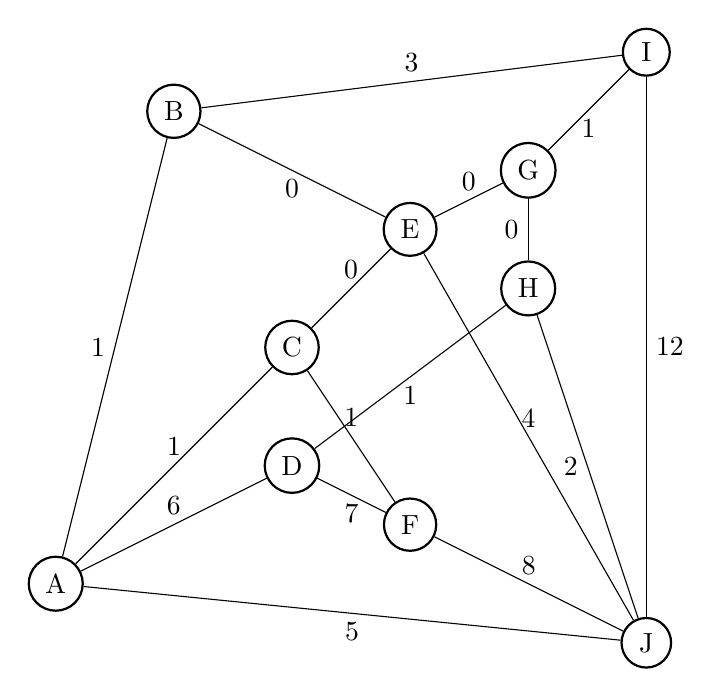
\begin{tikzpicture}[x=1.5cm, y=1.5cm, scale=1]
			\begin{scope}[every node/.style={circle,thick,draw}]
				\node (a) at (0,0) {A};
				\node (b) at (1,4) {B};
				\node (c) at (2,2) {C};
				\node (d) at (2,1) {D};
				\node (e) at (3,3) {E};
				\node (f) at (3,0.5) {F};
				\node (g) at (4,3.5) {G};
				\node (h) at (4,2.5) {H};
				\node (i) at (5, 4.5) {I};
				\node (j) at (5,-0.5) {J};
			\end{scope}
			\begin{scope}
				\path (a)
					edge node[left] {1} (b)
					edge node[above] {1} (c)
					edge node[above] {6} (d)
					edge node[below] {5} (j)
					;
				\path (b)
					edge node[above] {3} (i)
					edge node[below] {0} (e)
				;
				\path (c) 
					edge node[above] {0} (e)
					edge node[above] {1} (f)					
					;
				\path (d)
					edge node[below] {1} (h)
					edge node[below] {7} (f)					
					;
				\path (e)
					edge node[above] {0} (g)
					edge node[above] {4} (j)
					;
				\path (f)
					edge node[above] {8} (j)
					;
				\path (g)
					edge node[below] {1} (i)
					edge node[left] {0} (h)
					;
				\path (h)
					edge node[left] {2} (j)
					;
				\path (i)
					edge node[right] {12} (j)
					;					
			\end{scope}
		\end{tikzpicture}
		}\\
	Original Graph
	\end{minipage}
	\begin{minipage}{.3\textwidth}
		\centering
	\scalebox{0.8}{
		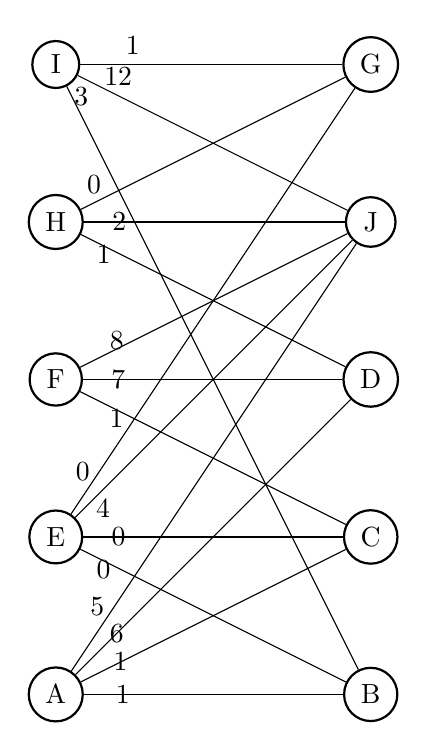
\begin{tikzpicture}[x=4cm, y=2cm, scale=1]
		\begin{scope}[every node/.style={circle,thick,draw}]
			\node (a) at (0,0) {A};
			\node (b) at (1,0) {B};
			\node (c) at (1,1) {C};
			\node (d) at (1,2) {D};
			\node (e) at (0,1) {E};
			\node (f) at (0,2) {F};
			\node (g) at (1,4) {G};
			\node (h) at (0,3) {H};
			\node (i) at (0, 4) {I};
			\node (j) at (1,3) {J};
		\end{scope}
		\begin{scope}
			\path (a)
			edge node[pos=0.15, ] {1} (b)
			edge node[pos=0.15, ] {1} (c)
			edge node[pos=0.15, ] {6} (d)
			edge node[pos=0.15, left] {5} (j)
			;
			\path (b)
			edge node[pos=0.95, above] {3} (i)
			edge node[pos=0.85, left] {0} (e)
			;
			\path (c) 
			edge node[pos=0.8, left] {0} (e)
			edge node[pos=0.8, left] {1} (f)					
			;
			\path (d)
			edge node[pos=0.85, left] {1} (h)
			edge node[pos=0.8, left] {7} (f)					
			;
			\path (e)
			edge node[pos=0.1, left] {0} (g)
			edge node[pos=0.1, below] {4} (j)
			;
			\path (f)
			edge node[pos=0.2, left] {8} (j)
			;
			\path (g)
			edge node[pos=0.8, above] {1} (i)
			edge node[pos=0.95, above] {0} (h)
			;
			\path (h)
			edge node[pos=0.2, left] {2} (j)
			;
			\path (i)
			edge node[pos=0.15, above] {12} (j)
			;					
		\end{scope}
	\end{tikzpicture}
	}\\
Bipartite-view
	\end{minipage}
\begin{minipage}{.3\textwidth}
	\centering
	$$
	\begin{matrix}
		&  B &  C&  D&  J&G \\ 
		A& 1 & 1 & 6 &  5 & -\\ 
		E& 0 & 0 & - &  4 & 0\\ 
		F& - & 1 & 7 &  8 & -\\ 
		H& - & - & 1 &  2 & 0\\ 
		I& 3 & - & - & 12 &1 
	\end{matrix}
	$$\\
	Matrix representation
\end{minipage}

Algorithm:
	\begin{equation}
		\begin{matrix}
			&&  B &  C&  D&  J&G \\ 
			&A& 1 & 1 & 6 &  5 & -\\ 
			*&E& \fbox{0} & 0 & - &  4 & 0\\ 
			&F& - & 1 & 7 &  8 & -\\ 
			*&H& - & - & 1 &  2 & \fbox{0}\\ 
			&I& 3 & - & - & 12 &1 
		\end{matrix}
		\xrightarrow{\Delta = 0.5}
		\begin{matrix}
			&&  B &  C&  D&  J&G \\ 
			&A& 1 & 1 & 6 &  5 & -\\ 
			*&E& \fbox{0} & 0 & - &  4 & 0\\ 
			&F& - & 1 & 7 &  8 & -\\ 
			*&H& - & - & 1 &  2 & \fbox{0}\\ 
			&I& 3 & - & - & 12 &1 
		\end{matrix}
	\end{equation}


\end{document}